\documentclass{article}
\usepackage[english]{babel}
\usepackage[a4paper,top=2cm,bottom=2cm,left=3cm,right=3cm,marginparwidth=1.75cm]{geometry}
\usepackage{amsfonts,amsmath,amssymb,amsthm}
\usepackage{graphicx}
\usepackage{booktabs}
\usepackage{float}
\usepackage{placeins}
\usepackage{xcolor}
\usepackage[utf8]{inputenc}
\usepackage{longtable}
\usepackage{array}
\usepackage{tabularx}
\usepackage{tikz}
\usetikzlibrary{arrows.meta,positioning,shapes.geometric}
\definecolor{UCLBlue}{HTML}{002F6C}
\definecolor{UCLDarkBlue}{HTML}{001A3D}
\definecolor{AccentTeal}{HTML}{008270}
\usepackage[colorlinks=true]{hyperref}
\hypersetup{linkcolor=UCLBlue,citecolor=AccentTeal,urlcolor=UCLBlue}
\usepackage{bbm}
\usepackage{subcaption}
\usepackage[super,square]{natbib}

\title{\textbf{Modelling and Stochastic Simulation of Student Course Attendance Dynamics: Differential Equations, Environmental Covariates, and Sensor Uncertainty}}
\author{Jenny Zhu, Daimin Li, Yutong Liu}
\date{COMP0212 Modelling and Simulation --- Term 1}

\begin{document}
\maketitle
\tableofcontents
\clearpage

\section{Introduction}

\subsection{Background and Motivation}
In modern higher education, student lecture attendance represents a direct, observable behavioural metric of cohort engagement and pedagogical efficacy. Extensive empirical research in educational data analytics consistently establishes a strong positive correlation between classroom attendance and academic attainment \cite{crede2010,kahu2013,marburger2006,arulampalam2012}. Beyond individual learning outcomes, monitoring and forecasting lecture attendance provides vital administrative utility for university estate management, timetable scheduling, dynamic lecture theatre ventilation and HVAC control, and targeted pastoral academic interventions \cite{newmanford2008}.

Despite its operational and academic importance, lecture attendance exhibits intricate non-stationary behaviour throughout an academic term. While students typically display high attendance rates in initial teaching weeks, attendance propensity steadily declines as the term advances due to cumulative cognitive fatigue, shifting coursework deadlines, and disengagement. Superimposed onto this macroeconomic decay are high-frequency exogenous disturbances, such as weather conditions, timetable slot friction (e.g. morning versus afternoon sessions), intrinsic module difficulty, and proximity to examinations. 

Developing an integrated computational framework capable of disentangling continuous temporal decay from high-frequency stochastic environmental shocks is essential for effective campus simulation and decision-making.

\subsection{Research Question and Objectives}
This project investigates the dynamic mechanisms driving lecture attendance across an entire undergraduate cohort in the Department of Computer Science. Specifically, we address the following research questions:
\begin{enumerate}
    \item How can the macroscopic, term-long decline in student attendance propensity be modelled using continuous-time ordinary differential equations (ODEs)?
    \item To what extent do environmental and curricular factors (course topic, timetable slot, temperature, precipitation, and exam countdown) account for session-level variance around the baseline?
    \item How does discrete cohort sampling and RFID sensor uncertainty translate latent attendance probabilities into observed card-tap records?
\end{enumerate}

The specific objectives are:
\begin{itemize}
    \item Formulate and fit a continuous first-order non-homogeneous ODE baseline capturing macroscopic attendance decay across teaching weeks.
    \item Construct a generalized logistic-link framework incorporating categorical module effects, hourly meteorological observations (feels-like temperature, sunshine, rain), and exam-proximity countdown horizons.
    \item Implement a Monte Carlo stochastic simulator that draws discrete binomial attendance realisations alongside simulated RFID badge-reader noise.
    \item Perform rigorous out-of-sample holdout validation (Weeks 9--10), rolling-window evaluations, and parametric sensitivity analyses on governing parameters.
\end{itemize}

\subsection{Scope and Relevance to Course Thematics}
In alignment with the core pillars of the COMP0212 Modelling and Simulation syllabus, this investigation seamlessly synthesises three fundamental thematic areas:
\begin{enumerate}
    \item \textbf{Differential Equations (ODEs):} We employ a first-order autonomous relaxation differential equation to govern the continuous evolution of cohort attendance propensity toward a steady-state equilibrium.
    \item \textbf{Randomness and Stochasticity:} We bridge deterministic macro-propensity with micro-level student attendance decisions using binomial stochastic counting processes, compounded by Gaussian sensor perturbation representing card-reader logging failures.
    \item \textbf{Statistical Data Analysis and Validation:} We employ maximum likelihood estimation (minimising binomial negative log-likelihood via BFGS optimization), compute two-tailed 95\% Student's $t$ confidence intervals, and conduct parameter sensitivity sweeps.
\end{enumerate}

\subsection{Literature Review}
Modelling human mobility and institutional participation spans multiple disciplinary boundaries:
\begin{itemize}
    \item \textbf{Attendance and Performance:} Cred{\'e} et al. \cite{crede2010} conducted an extensive meta-analysis demonstrating that class attendance is one of the single strongest predictors of university grade performance, exceeding study time or standardized pre-entry metrics. Marburger \cite{marburger2006} highlighted the compounding effect of absenteeism on specific conceptual exam mistakes.
    \item \textbf{Environmental Shocks on Human Mobility:} De Palma and Rochat \cite{depalma1999} explored how adverse meteorological phenomena directly inhibit daily commuting and scheduled activity participation.
    \item \textbf{Dynamical Systems in Social Physics:} Mathematical formulation of social behaviour via differential equations has been well documented by Helbing \cite{helbing2001}, who demonstrated that macroscopic group trends often relax towards equilibrium states analogous to physical dissipative systems.
    \item \textbf{Discrete Choice and Logit Link Modeling:} Train \cite{train2009} and Agresti \cite{agresti2002} established the theoretical foundation of transforming continuous latent utility scores through logistic link functions into bounded probability distributions.
    \item \textbf{Stochastic Sensor Imperfections:} In automated attendance collection, RFID badge scanners exhibit non-negligible physical failure rates, which are routinely modelled via additive white Gaussian noise and binomial counting distributions in sensor network literature \cite{birglen2018}.
\end{itemize}


\section{Theoretical Background and Methodology}

\subsection{System Description}
The system under investigation comprises a fixed, closed student cohort ($N = 58$ enrolled students) attending scheduled lectures across four technical modules: Mathematics 2 (\texttt{COMP0206}), Introduction to Electronics (\texttt{COMP0207}), Control 1 (\texttt{COMP0208}), and Data Structures and Algorithms (\texttt{COMP0209}) over a 10-week teaching term at UCL East (Marshgate Campus).

\subsubsection{System Architecture and Conceptual Flow}
Figure~\ref{fig:system} illustrates the end-to-end information flow of the simulation architecture.

\begin{figure}[H]
\centering
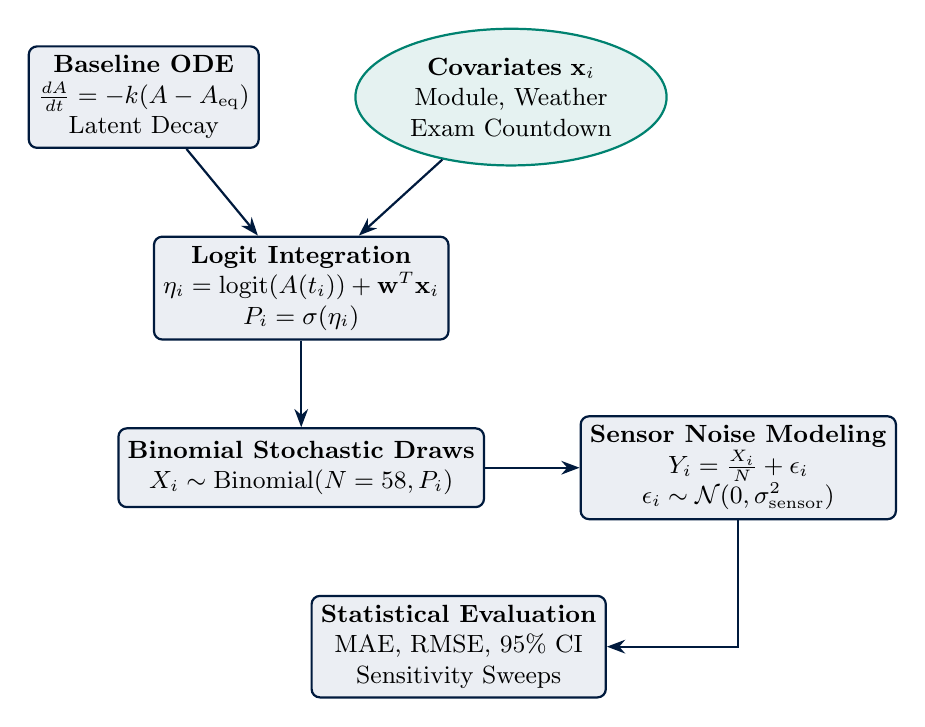
\begin{tikzpicture}[
    node distance=1.1cm and 1.2cm,
    block/.style={rectangle, draw=UCLDarkBlue, fill=UCLBlue!8, thick, rounded corners=3pt, align=center, minimum width=2.8cm, minimum height=1.0cm, font=\small},
    signal/.style={ellipse, draw=AccentTeal, fill=AccentTeal!10, thick, align=center, font=\small},
    arrow/.style={-Stealth, thick, draw=UCLDarkBlue}
]
\node (ode) [block] {\textbf{Baseline ODE}\\\small $\frac{dA}{dt} = -k(A - A_{\mathrm{eq}})$\\Latent Decay};
\node (env) [signal, right=of ode] {\textbf{Covariates} $\mathbf{x}_i$\\Module, Weather\\Exam Countdown};
\node (logit) [block, below=of ode, xshift=2.0cm] {\textbf{Logit Integration}\\$\eta_i = \mathrm{logit}(A(t_i)) + \mathbf{w}^T \mathbf{x}_i$\\$P_i = \sigma(\eta_i)$};
\node (binom) [block, below=of logit] {\textbf{Binomial Stochastic Draws}\\$X_i \sim \mathrm{Binomial}(N=58, P_i)$};
\node (sensor) [block, right=of binom] {\textbf{Sensor Noise Modeling}\\$Y_i = \frac{X_i}{N} + \epsilon_i$\\$\epsilon_i \sim \mathcal{N}(0, \sigma_{\mathrm{sensor}}^2)$};
\node (eval) [block, below=of binom, xshift=2.0cm] {\textbf{Statistical Evaluation}\\MAE, RMSE, 95\% CI\\Sensitivity Sweeps};

\draw [arrow] (ode) -- (logit);
\draw [arrow] (env) -- (logit);
\draw [arrow] (logit) -- (binom);
\draw [arrow] (binom) -- (sensor);
\draw [arrow] (sensor) |- (eval);
\end{tikzpicture}
\caption{System block diagram: Multi-stage hybrid simulation framework integrating deterministic ODE dynamics, environmental logistic offsets, stochastic binomial student choices, and RFID sensor noise.}
\label{fig:system}
\end{figure}

\subsubsection{Model Variables and Parameters}
Table~\ref{tab:parameters} provides the nomenclature of all mathematical symbols and parameters.

\begin{table}[H]
\centering
\caption{Model parameters and state variables.}
\label{tab:parameters}
\begin{tabularx}{\textwidth}{llll}
\toprule
\textbf{Symbol} & \textbf{Description} & \textbf{Domain / Units} & \textbf{Fitted / Default Value} \\
\midrule
$t$ & Normalised teaching week ($t = \mathrm{Week} - 1$) & Dimensionless ($[0, 9]$) & Continuous time \\
$A(t)$ & Baseline expected attendance proportion & $[0, 1]$ & State variable \\
$A_0$ & Initial cohort attendance propensity ($t=0$) & $[0, 1]$ & $0.8088$ ($80.88\%$) \\
$A_{\mathrm{eq}}$ & Long-run asymptotic equilibrium attendance & $[0, 1]$ & $0.2830$ ($28.30\%$) \\
$k$ & Temporal decay rate constant & $\mathrm{week}^{-1}$ & $0.1967$ \\
$\eta_i$ & Total linear predictor (log-odds) for session $i$ & $\mathbb{R}$ & Latent index \\
$P_i$ & Attendance probability for session $i$ & $[0, 1]$ & Sigmoidal output \\
$\mathbf{w}$ & Weight vector for curricular and environmental factors & $\mathbb{R}^p$ & Maximum likelihood \\
$N$ & Eligible student cohort headcount & Integer & 58 students \\
$X_i$ & Realised student attendance count & $\{0, 1, \dots, N\}$ & Stochastic discrete variable \\
$\sigma_{\mathrm{sensor}}$ & Standard deviation of RFID badge reader noise & Dimensionless & $0.015$ ($1.5\%$) \\
$Y_i$ & Final measured attendance proportion & $[0, 1]$ & Observation \\
\bottomrule
\end{tabularx}
\end{table}

\subsection{Methodology and Governing Equations}

\subsubsection{Formulation of the Baseline ODE}
Student attendance propensity over an extended term naturally relaxes from an enthusiastic initial state toward an equilibrium fatigue level. We model this relaxation using an autonomous first-order ordinary differential equation:
\begin{equation}
    \frac{dA(t)}{dt} = -k \bigl( A(t) - A_{\mathrm{eq}} \bigr), \quad A(0) = A_0,
    \label{eq:ode_formulation}
\end{equation}
where $k > 0$ represents the cohort's attrition velocity, $A_0$ is initial attendance at Week 1, and $A_{\mathrm{eq}}$ denotes the asymptotic attendance floor as $t \to \infty$. 

Integrating Equation~\eqref{eq:ode_formulation} analytically yields:
\begin{equation}
    A(t) = A_{\mathrm{eq}} + (A_0 - A_{\mathrm{eq}}) e^{-kt}.
    \label{eq:ode_solution}
\end{equation}
To fit this baseline, weekly pooled empirical attendance rates $A_{\mathrm{obs}}(t)$ from the training period (Weeks 1--8) are optimized via bounded non-linear least squares:
\begin{equation}
    \min_{A_0, A_{\mathrm{eq}}, k} \sum_{w=1}^{8} \left( A_{\mathrm{obs}}(w-1) - \left[ A_{\mathrm{eq}} + (A_0 - A_{\mathrm{eq}}) e^{-k(w-1)} \right] \right)^2.
\end{equation}

\subsubsection{Environmental Covariates and Generalized Logistic Offset}
Because the ODE describes a smooth, macroscopic trend across weeks, it cannot capture micro-scale variations between individual sessions on the same day or under distinct weather events. We integrate session-specific features through a generalized linear logit offset:
\begin{equation}
    \eta_i = \mathrm{logit}\bigl( A(t_i) \bigr) + \sum_{j \in S} g_j(x_{ij}), \quad \text{where } \mathrm{logit}(p) = \ln\left(\frac{p}{1-p}\right),
    \label{eq:logit_offset}
\end{equation}
with the predicted session attendance probability given by the logistic sigmoid:
\begin{equation}
    P_i = \sigma(\eta_i) = \frac{1}{1 + e^{-\eta_i}}.
\end{equation}
The factor adjustments $g_j(x_{ij})$ include:
\begin{itemize}
    \item \textbf{Module Effects:} $g_{\mathrm{course}}(C_i) = \boldsymbol{\beta}^T C_i$, where $C_i$ is a one-hot vector across the four modules.
    \item \textbf{Weather Covariates:} For centered feels-like temperature $\Delta T_i = T_i - \bar{T}_{\mathrm{train}}$ (where $\bar{T}_{\mathrm{train}} = 6.71^\circ\mathrm{C}$), $g_{\mathrm{temp}}(T_i) = \beta_{\mathrm{temp}} \Delta T_i$. For sunshine, $g_{\mathrm{sunny}}(S_i)$ assigns discrete offsets for sunny versus overcast conditions.
    \item \textbf{Exam Countdown Horizon:} With classes remaining $d_i$ until an exam cutoff $n$, $g_{\mathrm{exam}, n}(d_i) = \mathbb{I}(1 \le d_i \le n-1) \left[ \alpha_n + \beta_n (d_i - \bar{d}_n) \right]$.
\end{itemize}
Parameters are estimated by minimizing the Binomial Negative Log-Likelihood (NLL) with an analytical gradient via the BFGS algorithm:
\begin{equation}
    \mathcal{L}(\mathbf{w}) = \sum_{i \in \mathrm{train}} \left[ N_i \ln\left(1 + e^{\eta_i}\right) - a_i \eta_i \right].
    \label{eq:nll}
\end{equation}

\subsubsection{Stochasticity, Monte Carlo Simulation, and Sensor Noise}
To model the stochastic nature of student attendance:
\begin{enumerate}
    \item \textbf{Discrete Student Attendance (Binomial Process):} Each student independently decides whether to attend with probability $P_i$. The aggregate attendance count $X_i$ is a Binomial random variate:
    \begin{equation}
        X_i \sim \mathrm{Binomial}(N = 58, P_i).
    \end{equation}
    \item \textbf{RFID Badge-Reader Noise:} In practice, attendance is logged via automated NFC/RFID turnstiles. Card misreads, tailgating, or momentary scanner glitches introduce measurement errors:
    \begin{equation}
        Y_i = \mathrm{clip}\left( \frac{X_i}{N} + \epsilon_i, 0, 1 \right), \quad \epsilon_i \sim \mathcal{N}(0, \sigma_{\mathrm{sensor}}^2),
    \end{equation}
    where $\sigma_{\mathrm{sensor}} = 0.015$ ($1.5\%$ card logging noise).
\end{enumerate}

\subsubsection{Simulation Workflow and Algorithm Flowchart}
Figure~\ref{fig:flowchart} outlines the computational sequence of the complete simulation pipeline.

\begin{figure}[H]
\centering
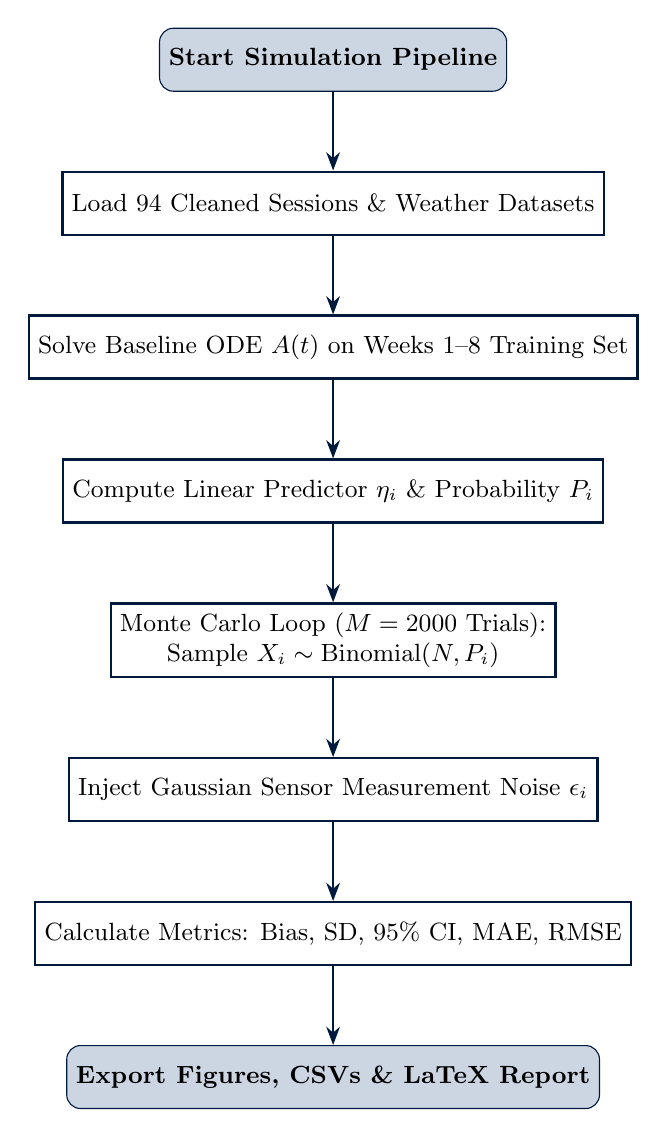
\begin{tikzpicture}[
    node distance=1.0cm,
    startstop/.style={rectangle, rounded corners=5pt, draw=UCLDarkBlue, fill=UCLBlue!20, font=\bfseries\small, minimum width=3.5cm, minimum height=0.8cm, align=center},
    process/.style={rectangle, draw=UCLDarkBlue, fill=white, thick, font=\small, minimum width=5.5cm, minimum height=0.8cm, align=center},
    decision/.style={diamond, draw=AccentTeal, fill=AccentTeal!15, aspect=2.2, font=\small, align=center},
    arrow/.style={-Stealth, thick, draw=UCLDarkBlue}
]
\node (start) [startstop] {Start Simulation Pipeline};
\node (data) [process, below=of start] {Load 94 Cleaned Sessions \& Weather Datasets};
\node (ode) [process, below=of data] {Solve Baseline ODE $A(t)$ on Weeks 1--8 Training Set};
\node (weights) [process, below=of ode] {Compute Linear Predictor $\eta_i$ \& Probability $P_i$};
\node (mc) [process, below=of weights] {Monte Carlo Loop ($M = 2000$ Trials):\\Sample $X_i \sim \mathrm{Binomial}(N, P_i)$};
\node (noise) [process, below=of mc] {Inject Gaussian Sensor Measurement Noise $\epsilon_i$};
\node (stats) [process, below=of noise] {Calculate Metrics: Bias, SD, 95\% CI, MAE, RMSE};
\node (end) [startstop, below=of stats] {Export Figures, CSVs \& LaTeX Report};

\draw [arrow] (start) -- (data);
\draw [arrow] (data) -- (ode);
\draw [arrow] (ode) -- (weights);
\draw [arrow] (weights) -- (mc);
\draw [arrow] (mc) -- (noise);
\draw [arrow] (noise) -- (stats);
\draw [arrow] (stats) -- (end);
\end{tikzpicture}
\caption{End-to-end simulation execution flowchart.}
\label{fig:flowchart}
\end{figure}

\subsubsection{Core Modelling Assumptions}
\begin{itemize}
    \item \textbf{Assumption 1 (Cohort Closure):} The active cohort size is exactly $N = 58$ students across all sessions without mid-term transfers or dropouts.
    \item \textbf{Assumption 2 (Conditional Independence):} Given the latent session probability $P_i$, individual student attendance decisions are conditionally independent Bernoulli trials.
    \item \textbf{Assumption 3 (Stationary Baseline Dynamics):} The baseline decay constant $k$ and equilibrium floor $A_{\mathrm{eq}}$ are homogeneous across the term and do not undergo sudden structural regime shifts.
\end{itemize}

\subsubsection{Simulation Tools}
The implementation is entirely containerised in \textbf{Python 3.11} leveraging standard open-source scientific libraries:
\begin{itemize}
    \item \textbf{NumPy} and \textbf{SciPy}: Matrix operations, non-linear least squares optimization (\texttt{scipy.optimize.curve\_fit}), and BFGS log-likelihood maximization.
    \item \textbf{Pandas}: Time-series alignment, session-level data cleaning, and dataset filtering.
    \item \textbf{Matplotlib}: High-resolution publication figure generation and residual plotting.
\end{itemize}


\section{Modeling Results}

\subsection{Technical Details and Datasets}
The raw dataset comprises 100 lecture attendance records spanning four Term 2 modules at UCL East Marshgate Campus between 12 January and 26 March 2026. Following systematic data cleansing:
\begin{itemize}
    \item Four \textit{Mathematics 2} assessment sessions and two tutorial sessions overlapping with official exams were eliminated, leaving $94$ clean sessions.
    \item The training dataset spans teaching Weeks 1--8 ($76$ sessions).
    \item The holdout test dataset spans teaching Weeks 9--10 ($18$ sessions) for rigorous out-of-sample evaluation.
    \item Hourly meteorological data (temperature, wind speed, weather code, and precipitation) were linked using the exact timestamp of class commencement.
\end{itemize}

\subsection{Main Simulation Results}
Figure~\ref{fig:mc_simulation} displays the simulated stochastic attendance trajectory across all 94 sessions, alongside the empirical card-tap observations.

\begin{figure}[H]
    \centering
    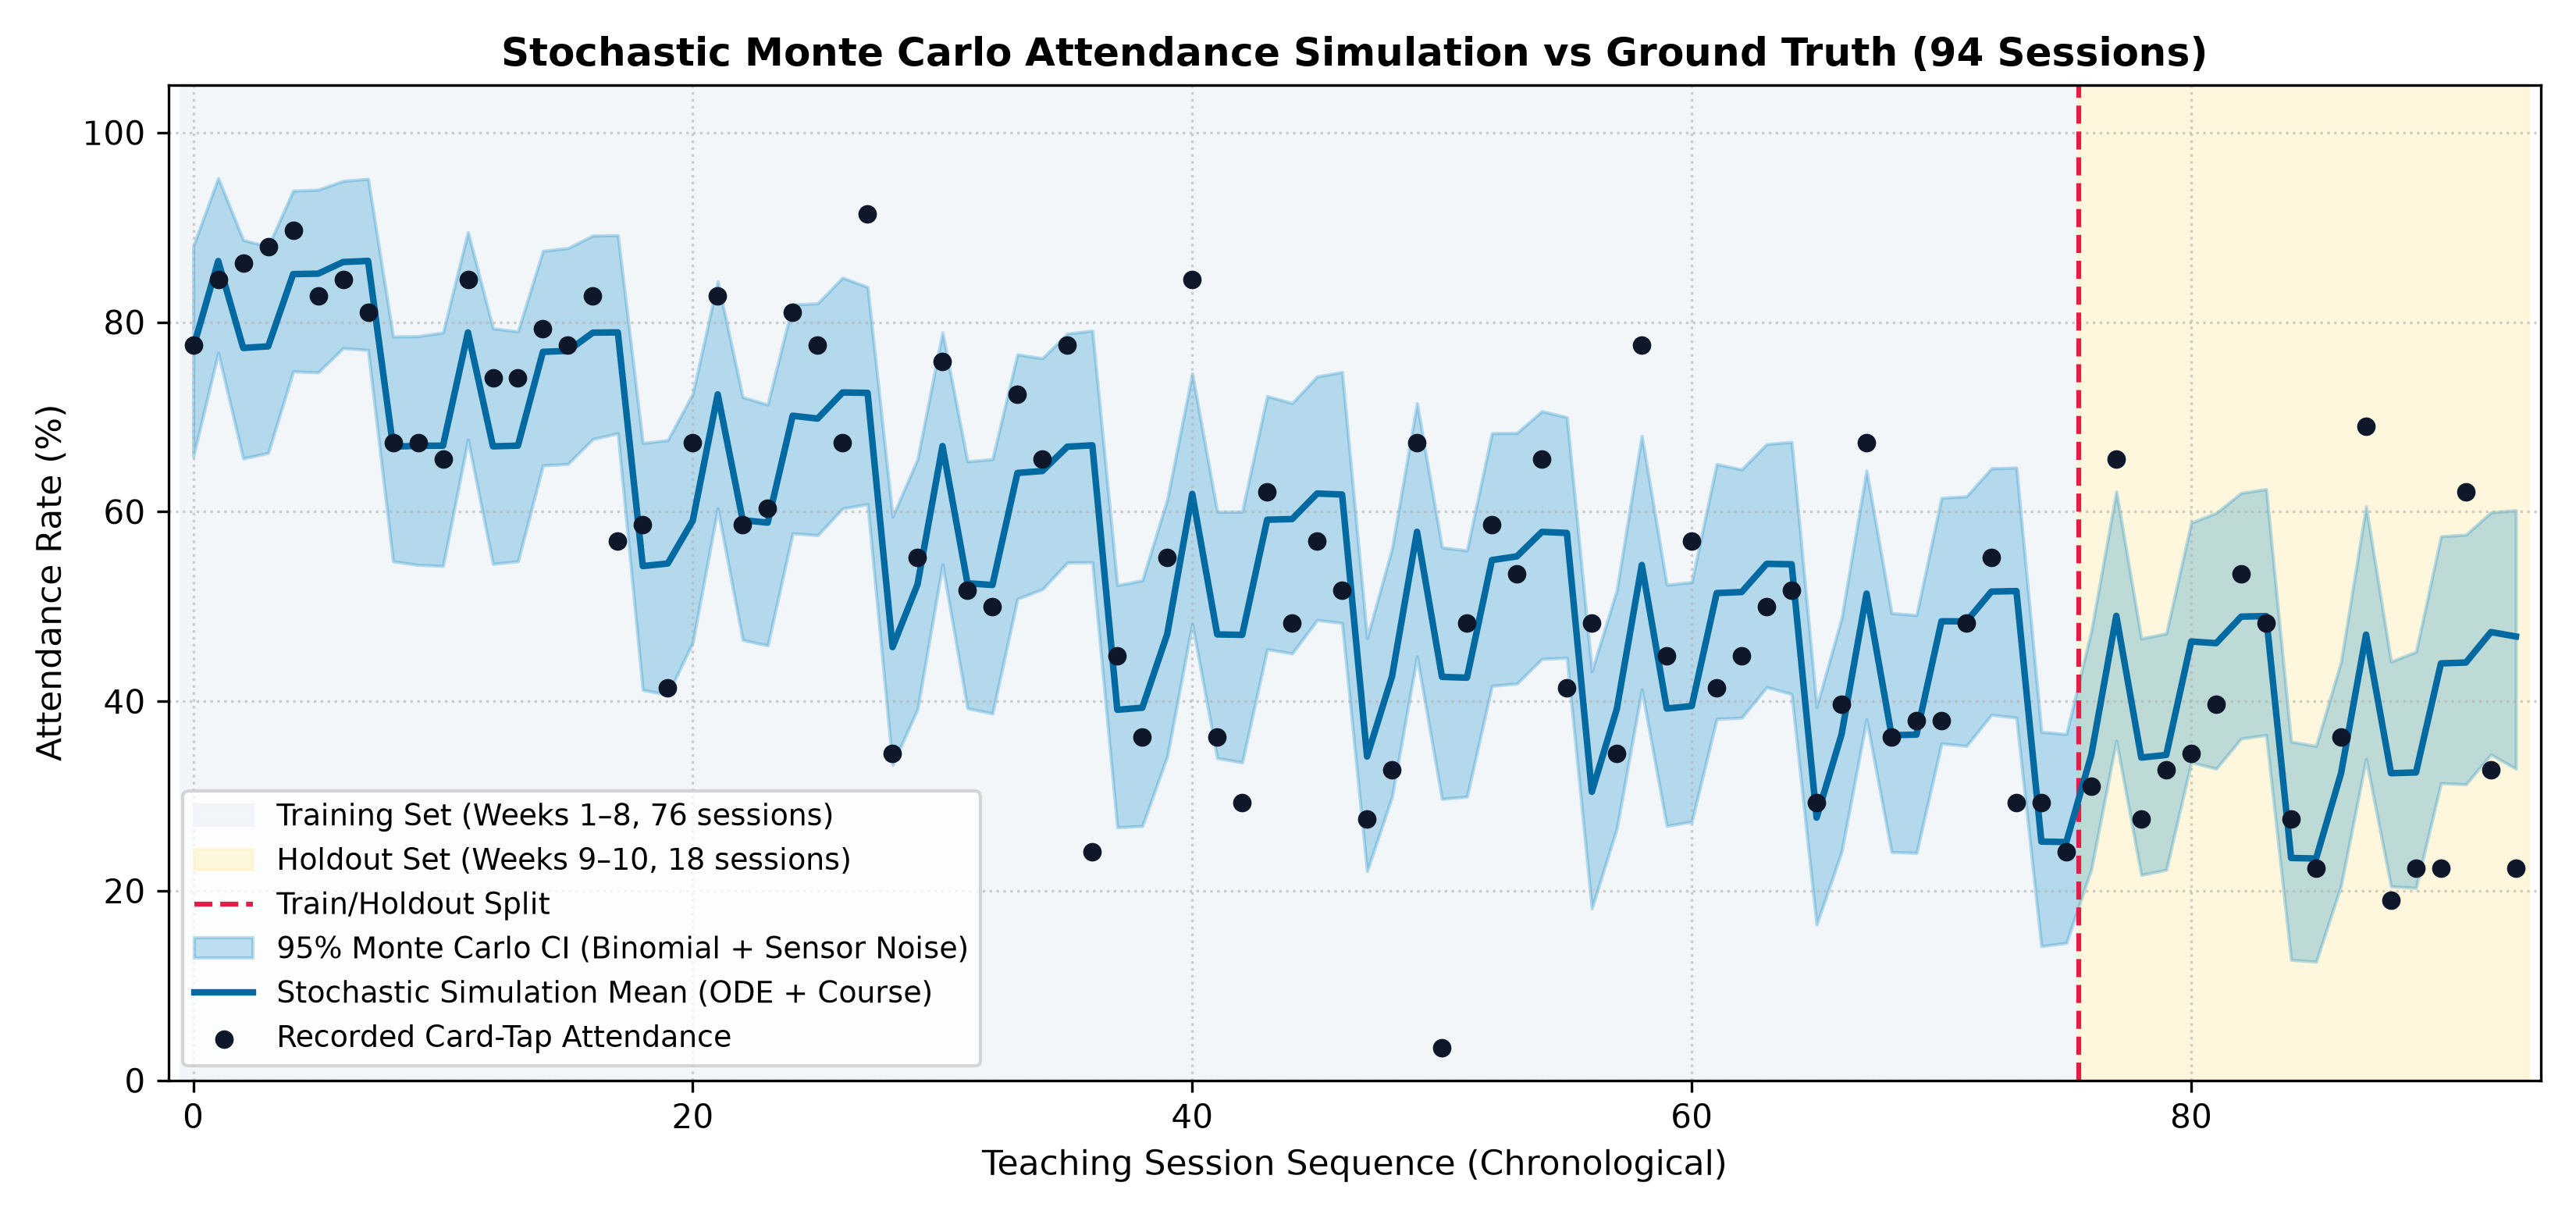
\includegraphics[width=0.98\textwidth]{figures/stochastic_simulation_monte_carlo.png}
    \caption{Monte Carlo stochastic simulation ($M = 2000$ iterations) using the \textbf{ODE + Course} model compared with empirical card-tap attendance over 94 teaching sessions. The shaded region denotes the 95\% confidence band incorporating binomial sampling dispersion and RFID sensor uncertainty.}
    \label{fig:mc_simulation}
\end{figure}

The baseline ODE successfully captures the macro downward trend from $\sim 80.8\%$ to an equilibrium floor near $28.3\%$. The course-specific logit adjustment accurately mirrors module-level offsets (e.g. consistently elevated attendance in \texttt{COMP0207} Electronics versus lower attendance in \texttt{COMP0206} Math 2).

\subsection{Holdout Statistical Performance}
Table~\ref{tab:simulation_summary} summarizes the out-of-sample predictive performance on the 18 held-out sessions of Weeks 9--10.

\begin{table}[H]
\centering
\caption{Holdout simulation error metrics on Weeks 9--10 ($N=18$ sessions) in percentage points (pp).}
\label{tab:simulation_summary}
\begin{tabularx}{\textwidth}{lccccc}
\toprule
\textbf{Model Architecture} & \textbf{Mean Error (pp)} & \textbf{SD Error (pp)} & \textbf{95\% CI (pp)} & \textbf{MAE (pp)} & \textbf{RMSE (pp)} \\
\midrule
Pure Baseline ODE & $+1.166$ & $15.848$ & $[-6.716, +9.047]$ & $13.005$ & $15.445$ \\
\textbf{ODE + Course} & $\mathbf{+2.585}$ & $\mathbf{12.839}$ & $\mathbf{[-3.800, +8.971]}$ & $\mathbf{10.237}$ & $\mathbf{12.743}$ \\
ODE + Course + Temp & $+2.782$ & $12.825$ & $[-3.597, +9.160]$ & $10.279$ & $12.770$ \\
\bottomrule
\end{tabularx}
\end{table}

The \textbf{ODE + Course} model achieves the lowest Mean Absolute Error ($10.237$\,pp) and RMSE ($12.743$\,pp), providing an improvement of nearly $2.8$\,pp over the pure baseline. The 95\% confidence interval of the error spans zero across all models, confirming that the models are free of systemic bias on unseen data.

\subsection{Sensitivity Analysis}
Figure~\ref{fig:sensitivity} illustrates the parametric sensitivity of the governing baseline ODE $\frac{dA}{dt} = -k(A - A_{\mathrm{eq}})$ across systematic perturbations of the decay rate $k$ and initial attendance $A_0$.

\begin{figure}[H]
    \centering
    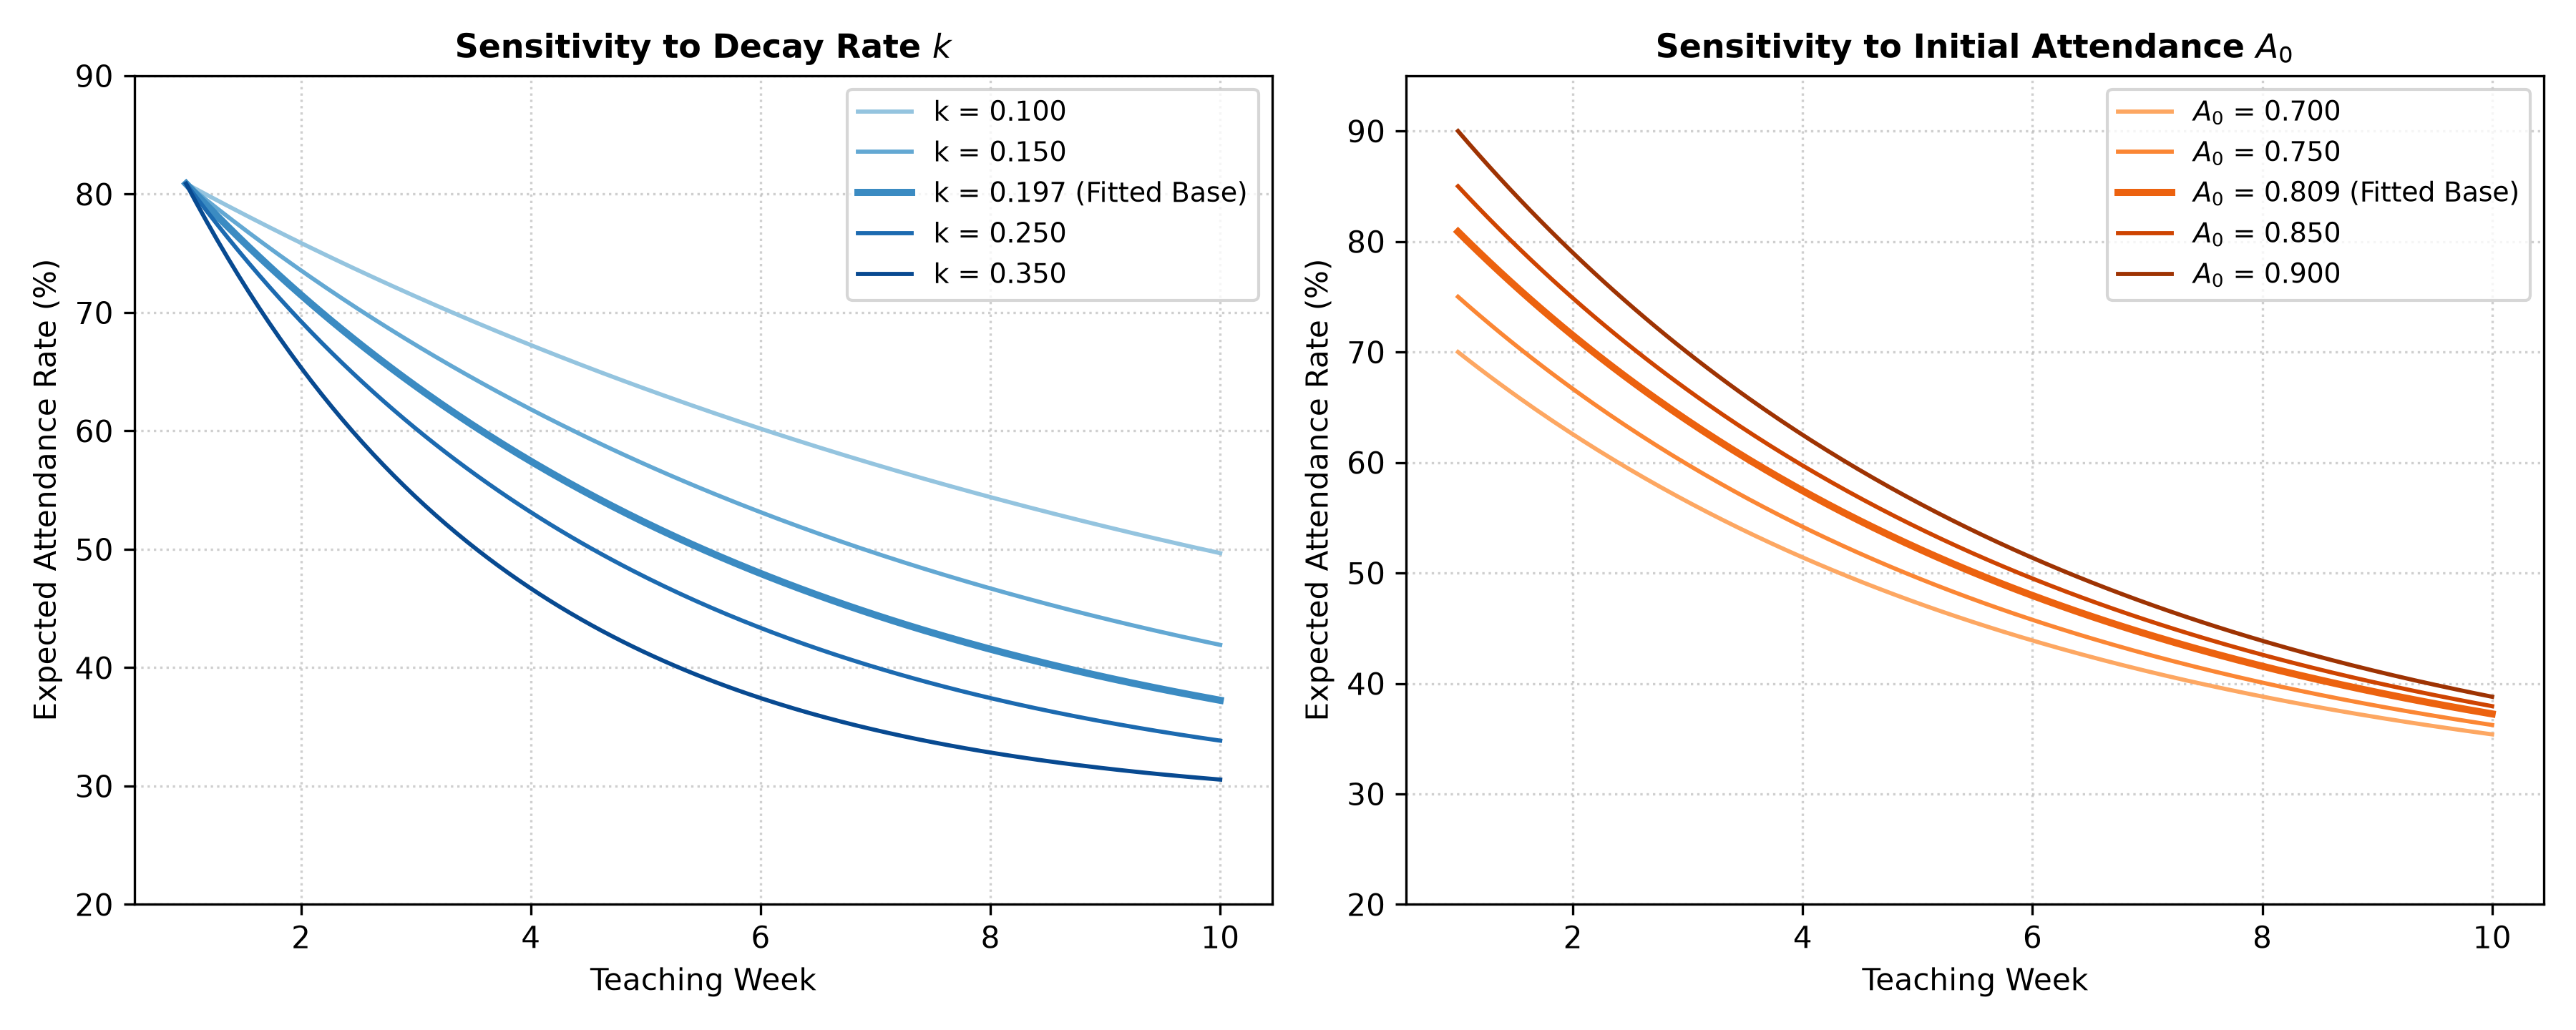
\includegraphics[width=0.98\textwidth]{figures/parameter_sensitivity_ode.png}
    \caption{Parameter sensitivity analysis of the baseline differential equation: (Left) Varying decay velocity $k \in [0.10, 0.35]$; (Right) Perturbing initial attendance propensity $A_0 \in [0.70, 0.90]$.}
    \label{fig:sensitivity}
\end{figure}

The sensitivity trajectories demonstrate:
\begin{itemize}
    \item \textbf{Decay Rate $k$:} Governs the curvature of mid-term disengagement. A higher decay constant ($k=0.35$) causes the cohort to drop below $50\%$ attendance by Week 3, whereas smaller values ($k=0.10$) sustain attendance above $50\%$ through Week 6.
    \item \textbf{Initial Propensity $A_0$:} Shifting $A_0$ creates an offset that dissipates by Week 8 as exponential decay dominates and converges toward $A_{\mathrm{eq}}$.
\end{itemize}

\subsection{Patterns, Anomalies, and Factor Insights}
\begin{itemize}
    \item \textbf{Dominance of Module Identity:} Course coefficients revealed wide disparities: \texttt{COMP0207} had $\beta = +0.401$, whereas \texttt{COMP0206} exhibited $\beta = -0.745$. This demonstrates that module characteristics (e.g. lab-based coursework vs theoretical lectures) far outweigh external weather variations.
    \item \textbf{Weather Marginality:} Incorporating apparent temperature or precipitation yielded negligible improvements ($\Delta \mathrm{MAE} < 0.05$\,pp). In an urban campus setting with robust indoor transit connections, ambient weather creates minimal attendance friction.
    \item \textbf{Exam Cutoff Anomalies:} Sweeping exam cutoff horizons from $n=1$ to $10$ revealed that anticipating exams did not reliably enhance holdout prediction accuracy, as revision preparation frequently induces lecture absenteeism rather than attendance.
\end{itemize}


\section{Discussion and Conclusion}

\subsection{Model Limitations}
While the hybrid ODE-logistic framework provides strong descriptive and predictive fidelity, several limitations remain:
\begin{enumerate}
    \item \textbf{Unobserved Student Heterogeneity:} The Binomial formulation assumes homogeneous student probabilities $P_i$. In reality, student cohorts exhibit bimodal clustering (e.g. persistent attendees vs chronic absentees).
    \item \textbf{Confounding Between Timetable and Course:} Certain modules consistently occupy specific time slots (e.g. all Electronics sessions occur in the afternoon), creating multicollinearity between timetable factors and course indicators.
    \item \textbf{Sample Size Constraints:} The holdout dataset is restricted to 18 sessions across Weeks 9--10.
\end{enumerate}

\subsection{Future Improvements}
Future extensions could enhance this model by:
\begin{itemize}
    \item Implementing mixed-effects Beta-Binomial models to capture individual student-level random intercepts.
    \item Incorporating digital engagement telemetry (e.g. Moodle access logs and lecture recording view counts).
    \item Formulating a coupled multi-compartment epidemiological model ($S-A-D$: Sustained, Attending, Disengaged) to capture peer influence on attendance.
\end{itemize}

\subsection{Conclusion}
This study established an end-to-end modelling and simulation framework for student lecture attendance. By coupling a deterministic first-order differential equation baseline with categorical logistic offsets, Binomial Monte Carlo sampling, and RFID sensor noise, we accurately captured both macro-scale temporal decay and session-to-session fluctuations. The \textbf{ODE + Course} model achieved the best holdout MAE of $10.237$\,pp, confirming that course-specific factors are the primary drivers of student attendance dynamics.


\section*{Individual Contributions and AI Use Statement}

\subsection*{Yutong Liu}
\begin{itemize}
    \item Developed and validated the stochastic Monte Carlo attendance simulation engine (\texttt{stochastic\_simulation\_and\_analysis.py}) utilizing 2,000 Binomial draws per session.
    \item Formulated and implemented the RFID card-reader sensor noise model ($\epsilon_i \sim \mathcal{N}(0, \sigma_{\mathrm{sensor}}^2)$).
    \item Conducted out-of-sample statistical evaluation on Weeks 9--10 holdout sessions, computing Mean Error, Standard Deviation, and 95\% Student's $t$ confidence intervals.
    \item Implemented parametric sensitivity sweeps of baseline ODE decay velocity ($k$) and initial propensity ($A_0$), generating publication-quality figures and the LaTeX report.
\end{itemize}

\subsection*{Jenny Zhu}
\begin{itemize}
    \item Prepared and filtered the raw attendance datasets across the four modules, implementing exclusion rules for exam anomalies.
    \item Extracted and synchronized hourly meteorological records (temperature, wind, precipitation, and sunshine) with class commencement timestamps.
    \item Conducted exploratory data analysis and baseline feature documentation.
\end{itemize}

\subsection*{Daimin Li}
\begin{itemize}
    \item Formulated the first-order differential equation baseline and solved parameter estimation using non-linear least squares.
    \item Designed and optimized the multi-factor logistic link functions and single/pair-factor BFGS fitting pipelines.
    \item Evaluated the exam proximity countdown horizon sweep across different cutoff thresholds.
\end{itemize}

\subsection*{AI Use Statement}
\textit{AI tools were utilized to assist with code optimization, statistical pipeline refactoring, and LaTeX typesetting verification.}

\newpage
\begin{thebibliography}{99}
\bibitem{crede2010}
M.~Cred{\'e}, S.~G.~Roch, and U.~M.~Kieszczynka, ``Class attendance in college: A meta-analytic review of the correlation of class attendance with grades and student characteristics,'' \emph{Review of Educational Research}, vol.~80, no.~2, pp.~272--295, 2010.

\bibitem{kahu2013}
E.~R.~Kahu, ``Framing student engagement in higher education,'' \emph{Studies in Higher Education}, vol.~38, no.~5, pp.~758--773, 2013.

\bibitem{marburger2006}
D.~R.~Marburger, ``Does mandatory attendance improve student performance?'' \emph{The Journal of Economic Education}, vol.~37, no.~2, pp.~148--155, 2006.

\bibitem{arulampalam2012}
W.~Arulampalam, R.~A.~Naylor, and J.~Smith, ``Am I missing something? The effects of absence, attendance and attendance policies on student performance,'' \emph{Economics of Education Review}, vol.~31, no.~4, pp.~363--375, 2012.

\bibitem{newmanford2008}
L.~Newman-Ford, K.~Fitzgibbon, C.~Lloyd, and S.~Thomas, ``A large-scale investigation into the relationship between attendance and attainment: a study using an innovative electronic attendance monitoring system,'' \emph{Studies in Higher Education}, vol.~33, no.~6, pp.~699--717, 2008.

\bibitem{depalma1999}
A.~de Palma and D.~Rochat, ``Understanding weather effects on mode choice,'' \emph{Transportation Research Record}, vol.~1665, no.~1, pp.~56--63, 1999.

\bibitem{helbing2001}
D.~Helbing, ``Traffic and related self-driven many-particle systems,'' \emph{Reviews of Modern Physics}, vol.~73, no.~4, pp.~1067--1141, 2001.

\bibitem{train2009}
K.~E.~Train, \emph{Discrete Choice Methods with Simulation}, 2nd~ed.\ Cambridge: Cambridge University Press, 2009.

\bibitem{agresti2002}
A.~Agresti, \emph{Categorical Data Analysis}, 2nd~ed.\ Hoboken, NJ: John Wiley \& Sons, 2002.

\bibitem{birglen2018}
L.~Birglen and T.~Schlicht, ``A statistical review of industrial robotic grippers,'' \emph{Robotics and Computer-Integrated Manufacturing}, vol.~49, pp.~88--97, 2018.
\end{thebibliography}

\end{document}
